% Created by tikzDevice version 0.12.4 on 2023-07-06 13:18:30
% !TEX encoding = UTF-8 Unicode
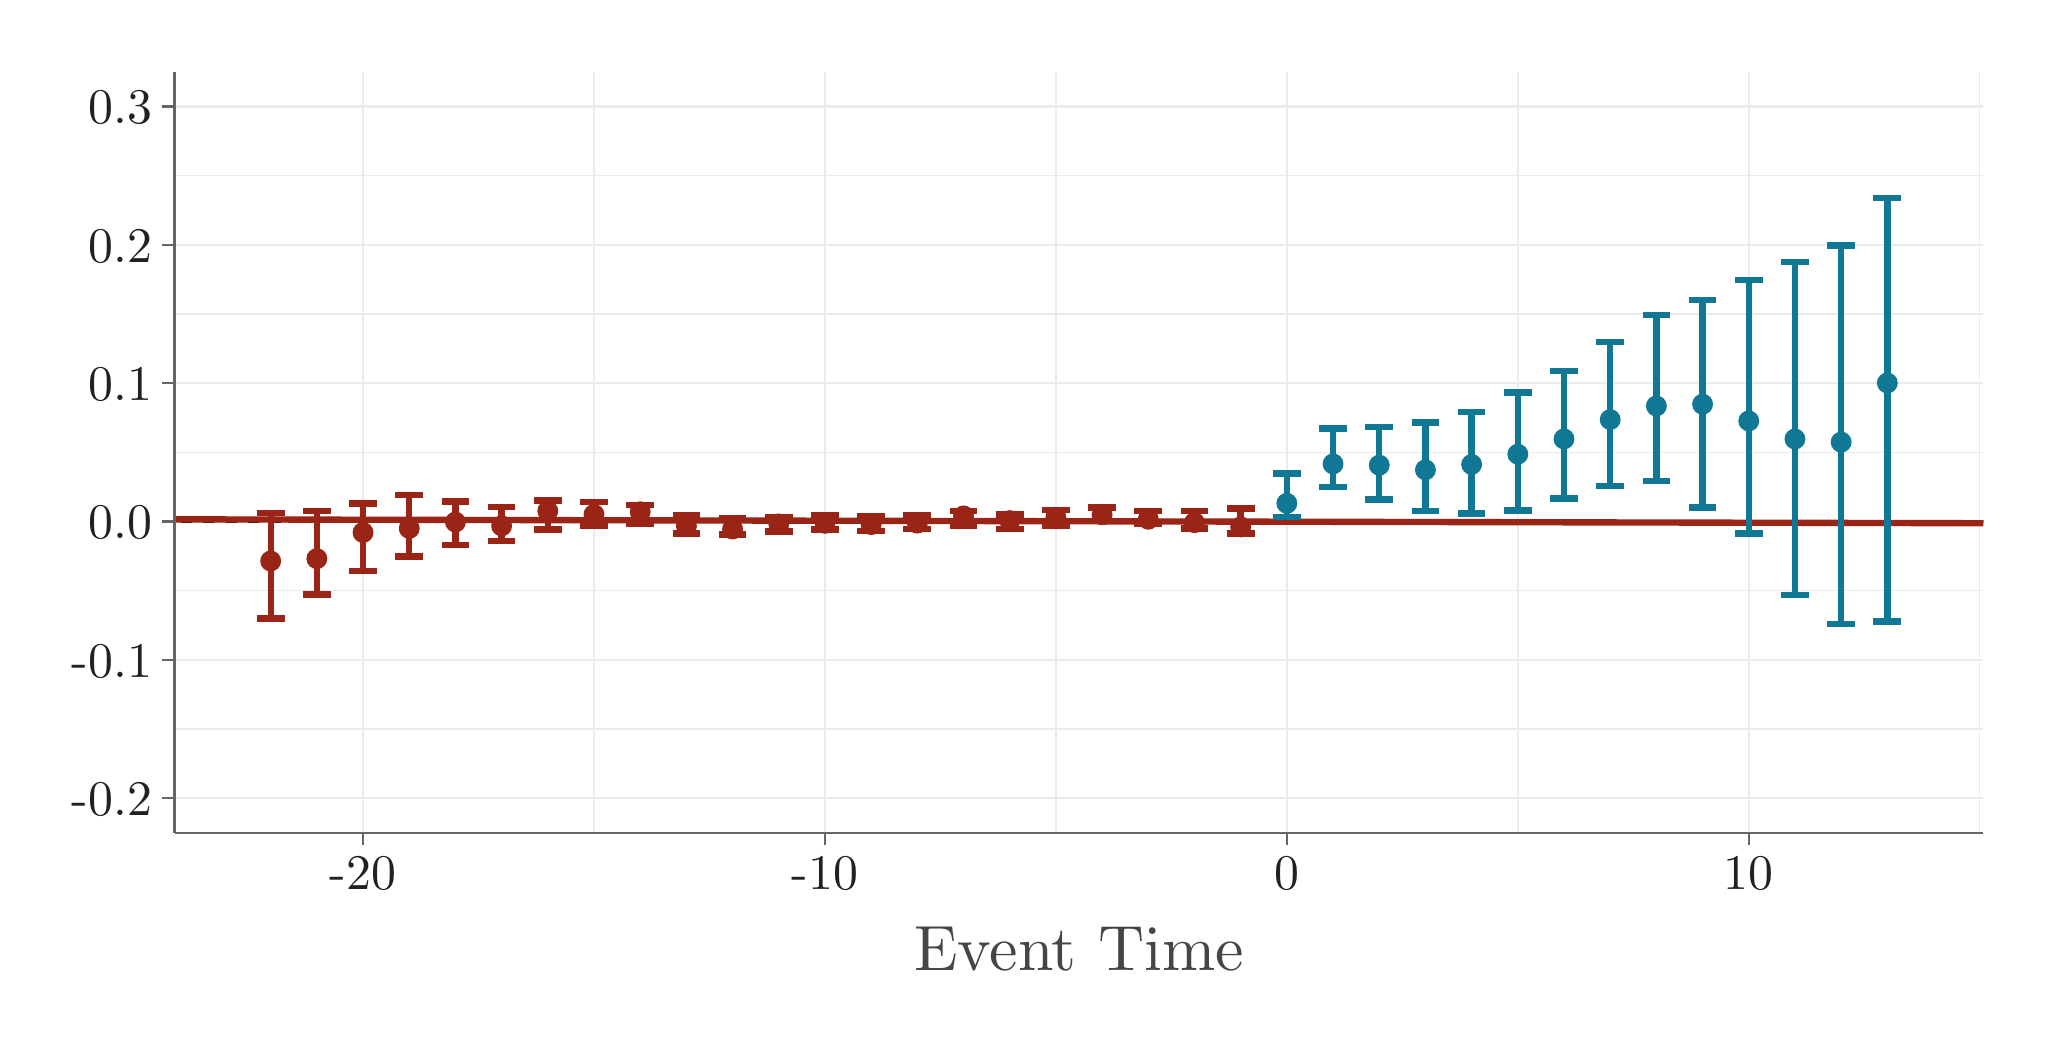
\begin{tikzpicture}[x=1pt,y=1pt]
\definecolor{fillColor}{RGB}{255,255,255}
\path[use as bounding box,fill=fillColor,fill opacity=0.00] (0,0) rectangle (722.70,361.35);
\begin{scope}
\path[clip] (  0.00,  0.00) rectangle (722.70,361.35);
\definecolor{fillColor}{RGB}{255,255,255}

\path[fill=fillColor] (  0.00, -0.00) rectangle (722.70,361.35);
\end{scope}
\begin{scope}
\path[clip] ( 53.09, 70.42) rectangle (706.70,345.35);
\definecolor{fillColor}{RGB}{255,255,255}

\path[fill=fillColor] ( 53.09, 70.42) rectangle (706.70,345.35);
\definecolor{drawColor}{gray}{0.92}

\path[draw=drawColor,line width= 0.5pt,line join=round] ( 53.09,107.91) --
	(706.70,107.91);

\path[draw=drawColor,line width= 0.5pt,line join=round] ( 53.09,157.90) --
	(706.70,157.90);

\path[draw=drawColor,line width= 0.5pt,line join=round] ( 53.09,207.89) --
	(706.70,207.89);

\path[draw=drawColor,line width= 0.5pt,line join=round] ( 53.09,257.87) --
	(706.70,257.87);

\path[draw=drawColor,line width= 0.5pt,line join=round] ( 53.09,307.86) --
	(706.70,307.86);

\path[draw=drawColor,line width= 0.5pt,line join=round] (204.64, 70.42) --
	(204.64,345.35);

\path[draw=drawColor,line width= 0.5pt,line join=round] (371.55, 70.42) --
	(371.55,345.35);

\path[draw=drawColor,line width= 0.5pt,line join=round] (538.46, 70.42) --
	(538.46,345.35);

\path[draw=drawColor,line width= 0.5pt,line join=round] (705.36, 70.42) --
	(705.36,345.35);

\path[draw=drawColor,line width= 0.9pt,line join=round] ( 53.09, 82.92) --
	(706.70, 82.92);

\path[draw=drawColor,line width= 0.9pt,line join=round] ( 53.09,132.91) --
	(706.70,132.91);

\path[draw=drawColor,line width= 0.9pt,line join=round] ( 53.09,182.89) --
	(706.70,182.89);

\path[draw=drawColor,line width= 0.9pt,line join=round] ( 53.09,232.88) --
	(706.70,232.88);

\path[draw=drawColor,line width= 0.9pt,line join=round] ( 53.09,282.87) --
	(706.70,282.87);

\path[draw=drawColor,line width= 0.9pt,line join=round] ( 53.09,332.85) --
	(706.70,332.85);

\path[draw=drawColor,line width= 0.9pt,line join=round] (121.19, 70.42) --
	(121.19,345.35);

\path[draw=drawColor,line width= 0.9pt,line join=round] (288.10, 70.42) --
	(288.10,345.35);

\path[draw=drawColor,line width= 0.9pt,line join=round] (455.00, 70.42) --
	(455.00,345.35);

\path[draw=drawColor,line width= 0.9pt,line join=round] (621.91, 70.42) --
	(621.91,345.35);
\definecolor{drawColor}{RGB}{0,0,0}

\path[draw=drawColor,line width= 0.9pt,dash pattern=on 4pt off 4pt ,line join=round] (-600.51,182.89) -- (1360.31,182.89);
\definecolor{drawColor}{RGB}{154,36,21}

\path[draw=drawColor,line width= 2.3pt,line join=round] (-600.51,185.10) -- (1360.31,180.87);
\definecolor{fillColor}{RGB}{154,36,21}

\path[draw=drawColor,line width= 0.4pt,line join=round,line cap=round,fill=fillColor] ( 87.81,168.63) circle (  3.57);

\path[draw=drawColor,line width= 0.4pt,line join=round,line cap=round,fill=fillColor] (104.50,169.48) circle (  3.57);

\path[draw=drawColor,line width= 0.4pt,line join=round,line cap=round,fill=fillColor] (121.19,178.93) circle (  3.57);

\path[draw=drawColor,line width= 0.4pt,line join=round,line cap=round,fill=fillColor] (137.88,180.41) circle (  3.57);

\path[draw=drawColor,line width= 0.4pt,line join=round,line cap=round,fill=fillColor] (154.57,182.71) circle (  3.57);

\path[draw=drawColor,line width= 0.4pt,line join=round,line cap=round,fill=fillColor] (171.26,181.33) circle (  3.57);

\path[draw=drawColor,line width= 0.4pt,line join=round,line cap=round,fill=fillColor] (187.95,186.74) circle (  3.57);

\path[draw=drawColor,line width= 0.4pt,line join=round,line cap=round,fill=fillColor] (204.64,185.45) circle (  3.57);

\path[draw=drawColor,line width= 0.4pt,line join=round,line cap=round,fill=fillColor] (221.34,186.42) circle (  3.57);

\path[draw=drawColor,line width= 0.4pt,line join=round,line cap=round,fill=fillColor] (238.03,181.26) circle (  3.57);

\path[draw=drawColor,line width= 0.4pt,line join=round,line cap=round,fill=fillColor] (254.72,180.18) circle (  3.57);

\path[draw=drawColor,line width= 0.4pt,line join=round,line cap=round,fill=fillColor] (271.41,182.03) circle (  3.57);

\path[draw=drawColor,line width= 0.4pt,line join=round,line cap=round,fill=fillColor] (288.10,182.24) circle (  3.57);

\path[draw=drawColor,line width= 0.4pt,line join=round,line cap=round,fill=fillColor] (304.79,181.79) circle (  3.57);

\path[draw=drawColor,line width= 0.4pt,line join=round,line cap=round,fill=fillColor] (321.48,182.31) circle (  3.57);

\path[draw=drawColor,line width= 0.4pt,line join=round,line cap=round,fill=fillColor] (338.17,184.92) circle (  3.57);

\path[draw=drawColor,line width= 0.4pt,line join=round,line cap=round,fill=fillColor] (354.86,183.23) circle (  3.57);

\path[draw=drawColor,line width= 0.4pt,line join=round,line cap=round,fill=fillColor] (371.55,184.37) circle (  3.57);

\path[draw=drawColor,line width= 0.4pt,line join=round,line cap=round,fill=fillColor] (388.24,185.32) circle (  3.57);

\path[draw=drawColor,line width= 0.4pt,line join=round,line cap=round,fill=fillColor] (404.93,183.72) circle (  3.57);

\path[draw=drawColor,line width= 0.4pt,line join=round,line cap=round,fill=fillColor] (421.62,182.50) circle (  3.57);

\path[draw=drawColor,line width= 0.4pt,line join=round,line cap=round,fill=fillColor] (438.31,180.94) circle (  3.57);
\definecolor{drawColor}{RGB}{16,120,149}
\definecolor{fillColor}{RGB}{16,120,149}

\path[draw=drawColor,line width= 0.4pt,line join=round,line cap=round,fill=fillColor] (455.00,189.48) circle (  3.57);

\path[draw=drawColor,line width= 0.4pt,line join=round,line cap=round,fill=fillColor] (471.70,203.71) circle (  3.57);

\path[draw=drawColor,line width= 0.4pt,line join=round,line cap=round,fill=fillColor] (488.39,203.26) circle (  3.57);

\path[draw=drawColor,line width= 0.4pt,line join=round,line cap=round,fill=fillColor] (505.08,201.57) circle (  3.57);

\path[draw=drawColor,line width= 0.4pt,line join=round,line cap=round,fill=fillColor] (521.77,203.53) circle (  3.57);

\path[draw=drawColor,line width= 0.4pt,line join=round,line cap=round,fill=fillColor] (538.46,207.24) circle (  3.57);

\path[draw=drawColor,line width= 0.4pt,line join=round,line cap=round,fill=fillColor] (555.15,212.73) circle (  3.57);

\path[draw=drawColor,line width= 0.4pt,line join=round,line cap=round,fill=fillColor] (571.84,219.73) circle (  3.57);

\path[draw=drawColor,line width= 0.4pt,line join=round,line cap=round,fill=fillColor] (588.53,224.65) circle (  3.57);

\path[draw=drawColor,line width= 0.4pt,line join=round,line cap=round,fill=fillColor] (605.22,225.30) circle (  3.57);

\path[draw=drawColor,line width= 0.4pt,line join=round,line cap=round,fill=fillColor] (621.91,219.24) circle (  3.57);

\path[draw=drawColor,line width= 0.4pt,line join=round,line cap=round,fill=fillColor] (638.60,212.72) circle (  3.57);

\path[draw=drawColor,line width= 0.4pt,line join=round,line cap=round,fill=fillColor] (655.29,211.60) circle (  3.57);

\path[draw=drawColor,line width= 0.4pt,line join=round,line cap=round,fill=fillColor] (671.98,232.96) circle (  3.57);
\definecolor{drawColor}{RGB}{154,36,21}

\path[draw=drawColor,line width= 2.3pt,line join=round] ( 82.80,185.91) --
	( 92.82,185.91);

\path[draw=drawColor,line width= 2.3pt,line join=round] ( 87.81,185.91) --
	( 87.81,147.84);

\path[draw=drawColor,line width= 2.3pt,line join=round] ( 82.80,147.84) --
	( 92.82,147.84);

\path[draw=drawColor,line width= 2.3pt,line join=round] ( 99.49,186.66) --
	(109.51,186.66);

\path[draw=drawColor,line width= 2.3pt,line join=round] (104.50,186.66) --
	(104.50,156.59);

\path[draw=drawColor,line width= 2.3pt,line join=round] ( 99.49,156.59) --
	(109.51,156.59);

\path[draw=drawColor,line width= 2.3pt,line join=round] (116.18,189.46) --
	(126.20,189.46);

\path[draw=drawColor,line width= 2.3pt,line join=round] (121.19,189.46) --
	(121.19,165.01);

\path[draw=drawColor,line width= 2.3pt,line join=round] (116.18,165.01) --
	(126.20,165.01);

\path[draw=drawColor,line width= 2.3pt,line join=round] (132.87,192.50) --
	(142.89,192.50);

\path[draw=drawColor,line width= 2.3pt,line join=round] (137.88,192.50) --
	(137.88,170.32);

\path[draw=drawColor,line width= 2.3pt,line join=round] (132.87,170.32) --
	(142.89,170.32);

\path[draw=drawColor,line width= 2.3pt,line join=round] (149.57,190.11) --
	(159.58,190.11);

\path[draw=drawColor,line width= 2.3pt,line join=round] (154.57,190.11) --
	(154.57,174.41);

\path[draw=drawColor,line width= 2.3pt,line join=round] (149.57,174.41) --
	(159.58,174.41);

\path[draw=drawColor,line width= 2.3pt,line join=round] (166.26,188.23) --
	(176.27,188.23);

\path[draw=drawColor,line width= 2.3pt,line join=round] (171.26,188.23) --
	(171.26,175.75);

\path[draw=drawColor,line width= 2.3pt,line join=round] (166.26,175.75) --
	(176.27,175.75);

\path[draw=drawColor,line width= 2.3pt,line join=round] (182.95,190.49) --
	(192.96,190.49);

\path[draw=drawColor,line width= 2.3pt,line join=round] (187.95,190.49) --
	(187.95,180.05);

\path[draw=drawColor,line width= 2.3pt,line join=round] (182.95,180.05) --
	(192.96,180.05);

\path[draw=drawColor,line width= 2.3pt,line join=round] (199.64,189.99) --
	(209.65,189.99);

\path[draw=drawColor,line width= 2.3pt,line join=round] (204.64,189.99) --
	(204.64,181.49);

\path[draw=drawColor,line width= 2.3pt,line join=round] (199.64,181.49) --
	(209.65,181.49);

\path[draw=drawColor,line width= 2.3pt,line join=round] (216.33,188.95) --
	(226.34,188.95);

\path[draw=drawColor,line width= 2.3pt,line join=round] (221.34,188.95) --
	(221.34,182.22);

\path[draw=drawColor,line width= 2.3pt,line join=round] (216.33,182.22) --
	(226.34,182.22);

\path[draw=drawColor,line width= 2.3pt,line join=round] (233.02,185.18) --
	(243.03,185.18);

\path[draw=drawColor,line width= 2.3pt,line join=round] (238.03,185.18) --
	(238.03,178.63);

\path[draw=drawColor,line width= 2.3pt,line join=round] (233.02,178.63) --
	(243.03,178.63);

\path[draw=drawColor,line width= 2.3pt,line join=round] (249.71,184.00) --
	(259.72,184.00);

\path[draw=drawColor,line width= 2.3pt,line join=round] (254.72,184.00) --
	(254.72,178.26);

\path[draw=drawColor,line width= 2.3pt,line join=round] (249.71,178.26) --
	(259.72,178.26);

\path[draw=drawColor,line width= 2.3pt,line join=round] (266.40,184.52) --
	(276.41,184.52);

\path[draw=drawColor,line width= 2.3pt,line join=round] (271.41,184.52) --
	(271.41,179.33);

\path[draw=drawColor,line width= 2.3pt,line join=round] (266.40,179.33) --
	(276.41,179.33);

\path[draw=drawColor,line width= 2.3pt,line join=round] (283.09,185.27) --
	(293.10,185.27);

\path[draw=drawColor,line width= 2.3pt,line join=round] (288.10,185.27) --
	(288.10,179.99);

\path[draw=drawColor,line width= 2.3pt,line join=round] (283.09,179.99) --
	(293.10,179.99);

\path[draw=drawColor,line width= 2.3pt,line join=round] (299.78,184.96) --
	(309.80,184.96);

\path[draw=drawColor,line width= 2.3pt,line join=round] (304.79,184.96) --
	(304.79,179.43);

\path[draw=drawColor,line width= 2.3pt,line join=round] (299.78,179.43) --
	(309.80,179.43);

\path[draw=drawColor,line width= 2.3pt,line join=round] (316.47,185.26) --
	(326.49,185.26);

\path[draw=drawColor,line width= 2.3pt,line join=round] (321.48,185.26) --
	(321.48,180.08);

\path[draw=drawColor,line width= 2.3pt,line join=round] (316.47,180.08) --
	(326.49,180.08);

\path[draw=drawColor,line width= 2.3pt,line join=round] (333.16,186.80) --
	(343.18,186.80);

\path[draw=drawColor,line width= 2.3pt,line join=round] (338.17,186.80) --
	(338.17,181.30);

\path[draw=drawColor,line width= 2.3pt,line join=round] (333.16,181.30) --
	(343.18,181.30);

\path[draw=drawColor,line width= 2.3pt,line join=round] (349.85,185.46) --
	(359.87,185.46);

\path[draw=drawColor,line width= 2.3pt,line join=round] (354.86,185.46) --
	(354.86,180.27);

\path[draw=drawColor,line width= 2.3pt,line join=round] (349.85,180.27) --
	(359.87,180.27);

\path[draw=drawColor,line width= 2.3pt,line join=round] (366.54,187.04) --
	(376.56,187.04);

\path[draw=drawColor,line width= 2.3pt,line join=round] (371.55,187.04) --
	(371.55,181.36);

\path[draw=drawColor,line width= 2.3pt,line join=round] (366.54,181.36) --
	(376.56,181.36);

\path[draw=drawColor,line width= 2.3pt,line join=round] (383.23,187.96) --
	(393.25,187.96);

\path[draw=drawColor,line width= 2.3pt,line join=round] (388.24,187.96) --
	(388.24,183.00);

\path[draw=drawColor,line width= 2.3pt,line join=round] (383.23,183.00) --
	(393.25,183.00);

\path[draw=drawColor,line width= 2.3pt,line join=round] (399.93,186.59) --
	(409.94,186.59);

\path[draw=drawColor,line width= 2.3pt,line join=round] (404.93,186.59) --
	(404.93,182.09);

\path[draw=drawColor,line width= 2.3pt,line join=round] (399.93,182.09) --
	(409.94,182.09);

\path[draw=drawColor,line width= 2.3pt,line join=round] (416.62,186.70) --
	(426.63,186.70);

\path[draw=drawColor,line width= 2.3pt,line join=round] (421.62,186.70) --
	(421.62,180.38);

\path[draw=drawColor,line width= 2.3pt,line join=round] (416.62,180.38) --
	(426.63,180.38);

\path[draw=drawColor,line width= 2.3pt,line join=round] (433.31,187.61) --
	(443.32,187.61);

\path[draw=drawColor,line width= 2.3pt,line join=round] (438.31,187.61) --
	(438.31,178.59);

\path[draw=drawColor,line width= 2.3pt,line join=round] (433.31,178.59) --
	(443.32,178.59);
\definecolor{drawColor}{RGB}{16,120,149}

\path[draw=drawColor,line width= 2.3pt,line join=round] (450.00,200.21) --
	(460.01,200.21);

\path[draw=drawColor,line width= 2.3pt,line join=round] (455.00,200.21) --
	(455.00,184.56);

\path[draw=drawColor,line width= 2.3pt,line join=round] (450.00,184.56) --
	(460.01,184.56);

\path[draw=drawColor,line width= 2.3pt,line join=round] (466.69,216.45) --
	(476.70,216.45);

\path[draw=drawColor,line width= 2.3pt,line join=round] (471.70,216.45) --
	(471.70,195.29);

\path[draw=drawColor,line width= 2.3pt,line join=round] (466.69,195.29) --
	(476.70,195.29);

\path[draw=drawColor,line width= 2.3pt,line join=round] (483.38,217.14) --
	(493.39,217.14);

\path[draw=drawColor,line width= 2.3pt,line join=round] (488.39,217.14) --
	(488.39,190.80);

\path[draw=drawColor,line width= 2.3pt,line join=round] (483.38,190.80) --
	(493.39,190.80);

\path[draw=drawColor,line width= 2.3pt,line join=round] (500.07,218.66) --
	(510.08,218.66);

\path[draw=drawColor,line width= 2.3pt,line join=round] (505.08,218.66) --
	(505.08,186.67);

\path[draw=drawColor,line width= 2.3pt,line join=round] (500.07,186.67) --
	(510.08,186.67);

\path[draw=drawColor,line width= 2.3pt,line join=round] (516.76,222.43) --
	(526.77,222.43);

\path[draw=drawColor,line width= 2.3pt,line join=round] (521.77,222.43) --
	(521.77,185.85);

\path[draw=drawColor,line width= 2.3pt,line join=round] (516.76,185.85) --
	(526.77,185.85);

\path[draw=drawColor,line width= 2.3pt,line join=round] (533.45,229.51) --
	(543.47,229.51);

\path[draw=drawColor,line width= 2.3pt,line join=round] (538.46,229.51) --
	(538.46,186.89);

\path[draw=drawColor,line width= 2.3pt,line join=round] (533.45,186.89) --
	(543.47,186.89);

\path[draw=drawColor,line width= 2.3pt,line join=round] (550.14,237.23) --
	(560.16,237.23);

\path[draw=drawColor,line width= 2.3pt,line join=round] (555.15,237.23) --
	(555.15,191.27);

\path[draw=drawColor,line width= 2.3pt,line join=round] (550.14,191.27) --
	(560.16,191.27);

\path[draw=drawColor,line width= 2.3pt,line join=round] (566.83,247.76) --
	(576.85,247.76);

\path[draw=drawColor,line width= 2.3pt,line join=round] (571.84,247.76) --
	(571.84,195.79);

\path[draw=drawColor,line width= 2.3pt,line join=round] (566.83,195.79) --
	(576.85,195.79);

\path[draw=drawColor,line width= 2.3pt,line join=round] (583.52,257.59) --
	(593.54,257.59);

\path[draw=drawColor,line width= 2.3pt,line join=round] (588.53,257.59) --
	(588.53,197.51);

\path[draw=drawColor,line width= 2.3pt,line join=round] (583.52,197.51) --
	(593.54,197.51);

\path[draw=drawColor,line width= 2.3pt,line join=round] (600.21,263.05) --
	(610.23,263.05);

\path[draw=drawColor,line width= 2.3pt,line join=round] (605.22,263.05) --
	(605.22,187.91);

\path[draw=drawColor,line width= 2.3pt,line join=round] (600.21,187.91) --
	(610.23,187.91);

\path[draw=drawColor,line width= 2.3pt,line join=round] (616.90,270.13) --
	(626.92,270.13);

\path[draw=drawColor,line width= 2.3pt,line join=round] (621.91,270.13) --
	(621.91,178.53);

\path[draw=drawColor,line width= 2.3pt,line join=round] (616.90,178.53) --
	(626.92,178.53);

\path[draw=drawColor,line width= 2.3pt,line join=round] (633.59,276.76) --
	(643.61,276.76);

\path[draw=drawColor,line width= 2.3pt,line join=round] (638.60,276.76) --
	(638.60,156.36);

\path[draw=drawColor,line width= 2.3pt,line join=round] (633.59,156.36) --
	(643.61,156.36);

\path[draw=drawColor,line width= 2.3pt,line join=round] (650.29,282.57) --
	(660.30,282.57);

\path[draw=drawColor,line width= 2.3pt,line join=round] (655.29,282.57) --
	(655.29,145.89);

\path[draw=drawColor,line width= 2.3pt,line join=round] (650.29,145.89) --
	(660.30,145.89);

\path[draw=drawColor,line width= 2.3pt,line join=round] (666.98,299.89) --
	(676.99,299.89);

\path[draw=drawColor,line width= 2.3pt,line join=round] (671.98,299.89) --
	(671.98,146.72);

\path[draw=drawColor,line width= 2.3pt,line join=round] (666.98,146.72) --
	(676.99,146.72);

\path[] ( 53.09, 70.42) rectangle (706.70,345.35);
\end{scope}
\begin{scope}
\path[clip] (  0.00,  0.00) rectangle (722.70,361.35);
\definecolor{drawColor}{gray}{0.40}

\path[draw=drawColor,line width= 0.9pt,line join=round] ( 53.09, 70.42) --
	( 53.09,345.35);
\end{scope}
\begin{scope}
\path[clip] (  0.00,  0.00) rectangle (722.70,361.35);
\definecolor{drawColor}{gray}{0.13}

\node[text=drawColor,anchor=base east,inner sep=0pt, outer sep=0pt, scale=  1.80] at ( 44.99, 76.72) {-0.2};

\node[text=drawColor,anchor=base east,inner sep=0pt, outer sep=0pt, scale=  1.80] at ( 44.99,126.71) {-0.1};

\node[text=drawColor,anchor=base east,inner sep=0pt, outer sep=0pt, scale=  1.80] at ( 44.99,176.69) {0.0};

\node[text=drawColor,anchor=base east,inner sep=0pt, outer sep=0pt, scale=  1.80] at ( 44.99,226.68) {0.1};

\node[text=drawColor,anchor=base east,inner sep=0pt, outer sep=0pt, scale=  1.80] at ( 44.99,276.67) {0.2};

\node[text=drawColor,anchor=base east,inner sep=0pt, outer sep=0pt, scale=  1.80] at ( 44.99,326.65) {0.3};
\end{scope}
\begin{scope}
\path[clip] (  0.00,  0.00) rectangle (722.70,361.35);
\definecolor{drawColor}{gray}{0.40}

\path[draw=drawColor,line width= 0.9pt,line join=round] ( 48.59, 82.92) --
	( 53.09, 82.92);

\path[draw=drawColor,line width= 0.9pt,line join=round] ( 48.59,132.91) --
	( 53.09,132.91);

\path[draw=drawColor,line width= 0.9pt,line join=round] ( 48.59,182.89) --
	( 53.09,182.89);

\path[draw=drawColor,line width= 0.9pt,line join=round] ( 48.59,232.88) --
	( 53.09,232.88);

\path[draw=drawColor,line width= 0.9pt,line join=round] ( 48.59,282.87) --
	( 53.09,282.87);

\path[draw=drawColor,line width= 0.9pt,line join=round] ( 48.59,332.85) --
	( 53.09,332.85);
\end{scope}
\begin{scope}
\path[clip] (  0.00,  0.00) rectangle (722.70,361.35);
\definecolor{drawColor}{gray}{0.40}

\path[draw=drawColor,line width= 0.9pt,line join=round] ( 53.09, 70.42) --
	(706.70, 70.42);
\end{scope}
\begin{scope}
\path[clip] (  0.00,  0.00) rectangle (722.70,361.35);
\definecolor{drawColor}{gray}{0.40}

\path[draw=drawColor,line width= 0.9pt,line join=round] (121.19, 65.92) --
	(121.19, 70.42);

\path[draw=drawColor,line width= 0.9pt,line join=round] (288.10, 65.92) --
	(288.10, 70.42);

\path[draw=drawColor,line width= 0.9pt,line join=round] (455.00, 65.92) --
	(455.00, 70.42);

\path[draw=drawColor,line width= 0.9pt,line join=round] (621.91, 65.92) --
	(621.91, 70.42);
\end{scope}
\begin{scope}
\path[clip] (  0.00,  0.00) rectangle (722.70,361.35);
\definecolor{drawColor}{gray}{0.13}

\node[text=drawColor,anchor=base,inner sep=0pt, outer sep=0pt, scale=  1.80] at (121.19, 49.93) {-20};

\node[text=drawColor,anchor=base,inner sep=0pt, outer sep=0pt, scale=  1.80] at (288.10, 49.93) {-10};

\node[text=drawColor,anchor=base,inner sep=0pt, outer sep=0pt, scale=  1.80] at (455.00, 49.93) {0};

\node[text=drawColor,anchor=base,inner sep=0pt, outer sep=0pt, scale=  1.80] at (621.91, 49.93) {10};
\end{scope}
\begin{scope}
\path[clip] (  0.00,  0.00) rectangle (722.70,361.35);
\definecolor{drawColor}{gray}{0.27}

\node[text=drawColor,anchor=base,inner sep=0pt, outer sep=0pt, scale=  2.31] at (379.90, 20.50) {Event Time};
\end{scope}
\end{tikzpicture}
